\chapter{A Chapter Title}
\chapterstyle{deposit}
% \begin{wbepi}{Deborah Land (2002)}
% \braces{Scholarship on school boards}... is rife with conclusions and recommendations based on personal experience, observations, and opinions. School board experts frequently rely on anecdotal evidence, rather than data from carefully designed research studies, to support their conclusions.
% \end{wbepi}


\section{Theoretical Underpinnings}
The question of the democratic nature of school boards has been central to the academic debate about school governance and politics for decades. On one hand, school boards embody the very concept of democratic local control of community public affairs—-giving local leaders the power to govern schools through the consent of community members. In practice, however, most school board elections have notoriously low turnout, with low levels of incumbent defeat, and few contested seats. School board members face little challenge, and school boards are increasingly constrained in their policy making ability by state and federal law \citep{RefWorks:318}. A literature has developed around this dilemma, but largely exists outside of the traditional political science literature surrounding elections, democracy, and public policy.

\subsection{Educational Governance Theory}
The 1970s saw the development of several theories of the role of school boards in making educational policy. Three major schools of thought, drawing on larger theories of democratic representation and urban politics, emerged from this period--dissatisfaction theory, continuous participation theory, and decision-output theory. A fourth theory--public choice theory--emerged in the late 80s as spatial models of voters and legislators began to gain prominence in the political science literature.

\textbf{Dissatisfaction Theory} is the first theory to emerge in this period and traces its roots back to  \citet{RefWorks:348}'s concept of critical elections. It describes an electoral system with relative stability and little involuntary incumbent turnover punctuated by periods of extreme citizen dissatisfaction, contentious elections, and incumbent defeats \citep{RefWorks:297,RefWorks:271}. Figure \ref{dissatdiag} displays the sequence of events in the model.\footnote{This diagram was adapted from \citep{RefWorks:243}} Dissatisfaction theory recently has been revived after a period of intense criticism by new work distinguishing between political and apolitical sources of board turnover. \citet{RefWorks:311} finds that if one ignores non-political cases of turnover--such as voluntary retirements, poor health, or a family move out of the district--then Dissatisfaction Theory can generate useful predictions. \citet{RefWorks:311} most recently used dissatisfaction theory to predict superintendent turnover. \citet{RefWorks:345} makes the case that, in order to evaluate how responsive school board elections are to democratic forces, it is necessary to conduct a study of many districts over several electoral cycles. Additionally, other studies fail to find meaningful elections with incumbent defeat because they lack a qualitative component--such as candidate interviews--to distinguish political turnover from from apolitical turnover \citep{RefWorks:311}. Despite the alignment with the \citet{RefWorks:348} theory of critical elections, and multiple empirical tests, Dissatisfaction Theory provides very little insight into the motives of board members, superintendents, and voters \citep{RefWorks:336}. Changing school board policy requires an inactive electorate to activate, challengers to run to replace incumbents in favor of the status quo, and a majority of board members to be defeated or change their positions in response to voter activity--prospectively and retrospectively--and ultimately a change in the school district superintendent or her policy preferences. In sum, Dissatisfaction Theory only explains aggregate behaviors and outcomes--turnover of school board members that leads to turnover of superintendents. It does not explain the motives of candidates to run for school board or of voters to vote for challengers, other than to say they do so out of dissatisfaction with the direction of the district. Thus, the political motives of board members, voters, and candidates are only crudely modeled by such a theory. 

\begin{center}
\begin{figure}[h!]
\caption{Dissatisfaction Theory}
\label{dissatdiag}
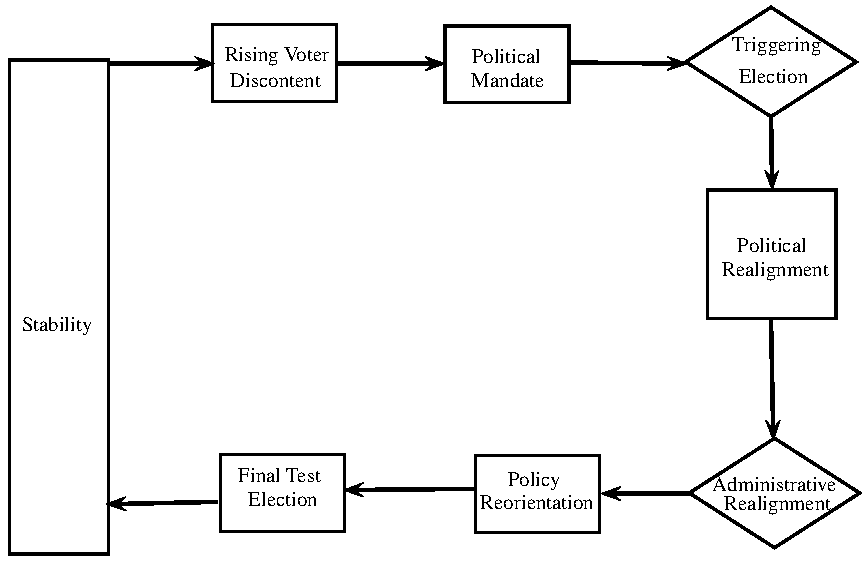
\includegraphics[width=.9\textwidth]{img/dissatdiagram}
\end{figure}
\end{center}

The strongest critique of Dissatisfaction Theory comes from \textbf{Continuous Participation Theory} which argues that policy and political turnover in local districts is largely illusory \citep{RefWorks:281}. The proponents of this theory argue that any changes in the makeup of the school board or the school board policies represent a true change in the preferences of the five to ten percent of the electorate who are constantly involved in educational policy at the local level. Spikes of participation may occur, but they are the direct result of the actions of this small public and the decisions that result from such periods of greater participation are in line with the views of the public that has been engaged all along. Recent studies on the capture of educational policymaking at the local level by teachers unions can trace its roots to this line of work \citep{RefWorks:207,RefWorks:320}. These works argue that teachers' unions function as a local elite in educational policymaking driving everything from school board candidate emergence, to voter turnout, to selection and replacement of district superintendents. Thus, when voter participation spikes or challenger candidates emerge it is not a reflection of broad dissatisfaction within the community, but of a concentrated effort to activate the electorate on behalf of the interests of the local elite. This line of argument has roots in the social science debate about power--particularly \citet{RefWorks:355}'s critique that power is not as elite concentrated as others like \citet{RefWorks:357} and \citet{RefWorks:360} posited, and the reply of \citet{RefWorks:356} that power is also about agenda setting and not just the outcomes of major decisions. However, since the studies developing this theory have only been cross-sectional single point in time studies, it has been impossible to disentangle the persistence of the local elite--a critical factor in evaluating whether school board politics are pluralist or elite dominated \citep{RefWorks:336}.

%For political science the issue of policy makers and elected officials responding more to the engaged members of the electorate is well studied territory from \citet{RefWorks:319} to \citet{RefWorks:354}.  

\textbf{Decision-Output Theory} is a derivative of Continuous Participation Theory. It argues that educational policy at the local level is largely undemocratic. However, policy is undemocratic not because of capture of the system by a single interest group, but rather because the electoral inputs available to citizens allow them only to determine who makes public policy and how much local tax revenue to raise in support of schools \citep{RefWorks:283}. Citizens are not able to truly determine education policy in these circumstances, but merely determine the constraints within which educational policy  makers must operate. In fact, it is the unelected district superintendent that dominates policymaking due to informational advantages and professional training. This reduces the issue dimensions in a school board election to a single fiscal dimension--to raise tax levies and  make new capital investments--but does not empower citizens to decide the substantive content of the community's students. 

Finally, \textbf{Public Choice Theory} is a late arrival to the study of school governance. The theory follows the rational choice tradition in economics and political science to model the behavior of individual actors and generate hypotheses about the resulting policy outcomes \citep{RefWorks:351}. In application to school boards \citet{RefWorks:336} identified two types of school board members--power and prestige candidates. Power candidates seek positions on the school board to change district policy and make decisions. Prestige candidates seek position to fulfill civic duty or to gain notoriety within the community. Additionally, all board members incur costs to information necessary for policy making that can be lessened by a district administrator, but have power and prestige candidates/board members have differing preferences for relying on the administrator for information. Applying this single dimension--power or prestige--to board members generates a number of expectations about the emergence of different types of candidates, electoral challenges, and policy changes within a community. 

\citet{RefWorks:336}'s theory has been extended and expanded upon since it was first posited \citep{RefWorks:339,RefWorks:340,RefWorks:243}. Figure \ref{wumodel} is the representation used by \citet{RefWorks:243} to depict the the most formalized and expanded version of the model. The model generates a number of interesting predictions based on the values of voters, board members, and changes in policy. For example, the theory expects that two types of low turnout elections are possible. In one scenario, voters and the board experience close policy alignment and thus the voter has little expected gain from casting a vote in support of a board member likely to win reelection and in support of the voter's preferences. In a different scenario voters are unhappy with board policies, but the policies are of low expected value to the voters and the expected benefits from voting are outweighed by the costs of voting. This nuance is missing from the other major theories discussed above and will be elaborated on further in the discussion of theory below.

It is important to note that Public Choice Theory has never been tested using election results from actual school board elections even in a limited fashion. 


Table \ref{sbtheory} summarizes the theories of school board politics. The next sections turn to the empirical work that supports and critiques these theories.

\begin{table}[h!]
\begin{center}
\begin{small}
\caption{Summarizing Major Theories}
\label{sbtheory}
\begin{tabular}{| p{.2\textwidth} | p{.5\textwidth} | p{.15\textwidth} |}
\hline
\textbf{Theory}  & \textbf{Description} & \textbf{Key Citations} \\ \hline
Dissatisfaction  & Long periods of equilibria in board elections punctuated by 
short periods of high turnover and high participation & \citet{RefWorks:297,RefWorks:271} \\ \hline
Continuous Participation (Competition) &The small percentage of voters who continuously participate in board 
elections have their preferences accurately reflected. Any spikes in participation are in line
with the wishes of these groups. & \citet{RefWorks:281} \\ \hline
Decision-Output (Responsiveness) & Undemocratic nature of school boards stems from the limited policy scope that board elections
control, namely the public can only vote on local tax revenue and the policy makers on the board,
who are constrained by federal and state policy. & \citet{RefWorks:283} \\ \hline
Public Choice Theory &  Challenges to incumbents arise based on 
policy choices of board members, voter preferences, and the expected payoffs associated with policy change. & \citet{RefWorks:336, RefWorks:340,RefWorks:243} \\ \hline
\end{tabular}
\end{small}
\end{center}
\end{table}

\subsection{Tying Back to Political Science}
All four of the above theories have deep roots in the political science literature, though few political scientists have taken up empirical work to evaluate the applicability of these theories to local special purpose governments. While this may seem of limited utility to the broader discipline beyond substantive interest in such governments, the study of special purpose governments like school districts presents a tremendous opportunity for political scientists to gain more leverage on key puzzles within the discipline.   

Understanding school boards provides an opportunity to evaluate what democratic policymaking looks like across a wide spectrum of levels of participation. While some variation exists in Congressional districts, school boards provide a much wider spectrum while playing an influential and often contentious role in the lives of citizens. Additionally, boards are a fascinating test of candidate emergence. Entry to school board office is relatively inexpensive and completely free of party gatekeepers--unlike legislative office. Where do candidates for office come from? Why do they serve? What motivates their decisions when partisan cues are unavailable? Is candidacy elite driven or individually motivated? 
 
Responsiveness to constituent preferences is seen as a critical to assessing the democratic nature of school boards. The literature here is mixed and unfortunately not empirically strong. This work began with Thomas Dye's 1967 study of 67 major urban districts which found no statistically significant difference in educational outcomes whether boards were appointed or elected \citep{RefWorks:224}. The question of whether elected boards were more accurately reflecting the preferences of the public was assessed by surveying the public and observing policy outcomes between school boards and the public \citep{RefWorks:226,RefWorks:331}. Surprisingly, school board members were found to be as responsive as other legislative bodies, despite their much narrower policy focus and nearness to constituents. This was due in part to the large percentage of unanimous decisions made by boards, around 90\%, which gave little official record of minority viewpoints. Additionally, at-large elected officials have less incentive to respond to individual constituent concerns, and lack of specialization on boards means that board members have little room to act independently of fellow board members. Unfortunately the generalizability of these findings is unknown due to the understandably small sample of eleven districts, and the age of the study. More recently Berkman and Plutzer leveraged national public opinion polling and US Census data on school district expenditures to correlate the responsiveness of school boards to estimates of local preferences for per pupil expenditures across nearly 8,000 US school districts \citep{RefWorks:332}
By this measure appointed school boards were found to be more responsive than their elected counterparts. This work, however, relies on imputed estimates of local preferences for spending and does not address the concern that appointed school boards may be the function of some political forces that also shape public preferences for school spending among many others.

Finally, boards provide an excellent lens for examining the way federalism plays out in local policy making. The history of school boards has been one of receding local control \citep{RefWorks:220}. Despite this, great variation in the authority, financial independence, and political activism of school boards exists--much more than the variation available among states vis-a-vis the federal government. Thus, school boards provide an interesting window into understanding a whole manner of other such intergovernmental relationships and their response to policy shocks, fiscal constraint, and changes in policy authority.

%Finally, boards provide an interesting test of government structure. Boards appoint an executive and make decisions by vote--often on recommendations made by the executive. At the same time, they have local authority over their school district, but are increasingly fiscally dependent on the state and federal government for funding. They are subject to the requirements of two bureaucratic entities--state and federal departments of education--in order to receive funds and subject to the whims of the state legislature where they often represent a state's single biggest budget item. Finally, they compete with one another for resources, and with other local governments for aid, capacity, and support from other levels of government. 

\section{Empirical Work}
In the last forty years there have been numerous studies of school boards. However, these studies have tended to be isolated from one another and not part of a cohesive research literature--many of them not tied to any of the major theories discussed above. The most comprehensive and widely cited review of the literature summarizes it as:
\begin{quote}
\begin{singlespace}
...rife with conclusions and recommendations based on personal experience, observations, and opinions. School board experts frequently rely on anecdotal evidence, rather than data from carefully designed research studies, to support their conclusions \citep[ p.265]{RefWorks:312}
\end{singlespace}
\end{quote}
\vspace{-6pt}
%\citet[p.265-267]{RefWorks:312} identifies at least five major issues with the research on school boards:
%\vspace{-6pt}% only necessary in double space environment
%\begin{enumerate}
%\setlength\itemsep{-6pt}
%\item Most research affiliated with organizations that develop training for school boards
%\item Failure to operationalize key variables like board effectiveness, governing behaviors, and obligations and responsibilities of school boards
%\item Too narrow of a focus on student test scores as a measurement of student achievement
%\item School boards not treated as an independent unit of district leadership distinct from superintendents
%\item Lack of conceptual models on the relationship between board activities and school and student outcomes
%\end{enumerate}
%\vspace{-6pt}

Despite these stated deficiencies, a scattering of excellent studies exist across disciplines that fall into the theoretical traditions outlined in Table \ref{sbtheory}. To move forward, the literature needs to focus on components of the questions that school boards raise so that a research literature can be constructed that builds on prior work and informs theory \citep{RefWorks:191}. That existing work is outlined here and can be loosely organized into surveys of school board members, questions of board politics, and board and superintendent relationships.

\subsection{Surveys of School Board Members}

Although school board membership is perhaps the most commonly held elected office in America, little is known about who holds these offices nationwide or how members are selected. Previously, the US Census Bureau provided this information by taking a census of all elected officials in the US. The Census Bureau was required under Title 13, United States Code Section 161 to take a census of all governmental bodies in the country at 5 year intervals. This began in 1957, with the census aimed at reporting on government organization, public employment, and government finance \citep{RefWorks:324}. The report on Popularly Elected Officials includes information on the number of elected officials per governing board or form of government, demographics of these elected officials, compensation, and their location \citep{RefWorks:325}. Unfortunately, after 1992 the Census of Governments no longer reported on elected officials directly due to budget cuts. This left scholars without any systematic data on who serves on school boards, how many school board members are active in the US, or how school boards are organized across the country. 

Partially in response to this the National School Boards Association (NSBA) commissioned a nationwide survey of school board members to fill the gap \citep{RefWorks:321}.\footnote{Another early survey came from Public Agenda \citep{RefWorks:330}.} Almost ten years later a second survey was taken to follow up \citep{RefWorks:322}. In addition to these national efforts, several smaller surveys of school board members have been conducted 
to address the needs of a particular topic \citep[see][]{RefWorks:264,speer1998reaching,RefWorks:311,RefWorks:328}. The utility of such surveys has been criticized because they rely on member self-reports and are only a single snapshot in time  \citep{RefWorks:327}. Any sense of temporal variation is derived from asking respondents to recollect past events such as elections, retirements, or board strife. Others believe that little can be learned from surveys that cannot be learned from other methods that provide additional information--such as in-depth interviews and observations \citep{RefWorks:329}
School board surveys, however, are underdeveloped compared to surveys of teachers for example, and thus criticism of them is premature \citep{RefWorks:312}. They are an important part of the mixed methods strategy necessary to untangle the complexity of the dynamics of school board politics and policy and to fill the gap left by the discontinuation of the Census report.

Since these criticisms, a number of excellent surveys have been conducted that have greatly increased our knowledge about many aspects of school board service--including who serves on school boards and how boards operate. Table \ref{sbsurveys2} summarizes the major surveys in the field and their key findings about the political nature of school boards. 


\begin{small}
\begin{singlespace}
\begin{longtable}{| p{.125\textwidth} | p{.725\textwidth} | p{.125\textwidth}|}
\hline

\caption{Key Findings of School Board Surveys} 
\label{sbsurveys2}\\ \hline
\textbf{Survey}  & \textbf{Findings} & \textbf{Sample} \\ \hline \endhead
\citet{RefWorks:321}  &  \vspace{-6mm} \begin{itemize} \setlength\itemsep{-2pt}
\item Over 90\% of boards are elected 
\item Board elections unlikely to be competitive \item Mean board tenure is 6.7 years 
\item Boards self identify as moderate or conservative, only 1 in 5 self-identify as liberal 
\end{itemize} \vspace{-4mm} & National \\ \hline
\citet{RefWorks:264} & \vspace{-6mm} \begin{itemize} \setlength\itemsep{-2pt}
\item Board conflict on decisions more 
common in urban and rural districts \item Conflict more common on large boards, boards with single-member district elections, 
and boards in active interest group environments \item Ideological diversity increases conflict, racial diversity correlates 
with lower conflict \item Professionalization leads to less division 
\end{itemize} \vspace{-4mm} & California \\ \hline
\citet{RefWorks:322} & \vspace{-6mm} \begin{itemize}
\setlength\itemsep{-2pt}\item 73.9\% of board members spent less than \$1,000
to be elected, 87\% spent less than \$5,000 \item 44\% described their last election as ``very easy'' \item Boards and 
superintendents agree on district priorities, disagree on how to evaluate performance of superintendents
\end{itemize} \vspace{-4mm}
& National \\ \hline
\citet{speer1998reaching} & \vspace{-6mm} \begin{itemize}
 \setlength\itemsep{-2pt}\item Superintendents and boards that have good relations are correlated with high student achievement \end{itemize} \vspace{-4mm} & National \\ \hline
\citet{RefWorks:311} & \vspace{-6mm} \begin{itemize} \setlength\itemsep{-2pt}\item Some evidence that politically driven board turnover leads to district administrator turnover \item Community values, citizen participation in elections, board values, and district policy are major variables and difficult to quantify even with survey methods
 \end{itemize} \vspace{-4mm}& Washington\\ \hline
\citet{RefWorks:333} &  \vspace{-6mm} \begin{itemize} \setlength\itemsep{-2pt}
\item 58\% of board members are employed full time outside of board service \item Business and commerce (23\%), followed by education (17\%) are the most common board member occupations \item Boards are fiscally conservative (50\%) or moderate (41\%) \item Boards are divided on social issues, 30\% conservative and 30\% liberal, 40\% moderate \item Board members self-identify as 44\% Republican and 44\% Democrat \item 66\% of members anticipate running for re-election \item Only 17\% anticipate running for a higher office--typically city council in an urban area 
\end{itemize} \vspace{-4mm} & California \\ \hline
\citet{RefWorks:328} & \vspace{-6mm} \begin{itemize} \setlength\itemsep{-2pt} 
\item After controlling for student 
background and school characteristics, boards matter for student outcomes \item Key to success is boards' involvement of
school team and parents in decision making
\end{itemize} \vspace{-4mm} & Netherlands \\ \hline  
\end{longtable}
\end{singlespace}
\end{small}

Immediately some key information seems to be missing from the findings in Table \ref{sbsurveys2}. Just a few examples: First, how common are ideologically divided boards? Second, what issues do candidates campaign on? How frequent are divisive campaigns in communities? How do board members perceive their electorate? And what interest groups play a vital role in the decisions taken up by and choices made by the school board?


%Surveys in 1997, 1998 ASBJ and Virginia Polytechnic

\subsection{Politics of School Boards}

While the descriptive studies have asked a few questions about the political aspect of school boards--chiefly about self-reported views of seat competitiveness and desire to seek re-election--little can be learned from such snapshots about the causes of electoral competition and the outcomes of incumbent success or defeat. Despite the staggering number of school board elections held annually in the United States, little systematic analysis of board elections has been conducted due to the significant challenge in collecting official records of election results at the school district or county level. The fact that the overwhelming majority of school board elections are non-partisan affairs about specific local issues also contributes--making it hard to identify unifying issues that board races focus on.

Despite the dearth of readily accessible data and obvious ideological identifiers like party affiliation, some quality scholarship has emerged applying the four theoretical frameworks in Table \ref{sbtheory} to school boards. These studies can be grouped by which facet of school board political activity they focus on--the electoral system, the outcome of board elections, board policy making, or political relations of boards with other governmental bodies. 

\subsubsection{Electoral Rules}
There are two types of studies that look at the way school board elections are structured. First, there are studies of how boards are selected--including studies of appointment, elections, and the implications of at-large electoral districts compared to sub-district elections. Single-member districts--predominantly in large urban centers--are correlated with increased racial diversity of school boards to align more closely with the communities they serve \citep{RefWorks:195,RefWorks:238}. This is important because surveys have demonstrated boards are often much less diverse than the communities they serve \citep{RefWorks:321,RefWorks:322}. Other work has explored how different election rules can influence the equality of school board representation across dimensions such as race, gender, and community values \citep{RefWorks:241,RefWorks:238}. Second, most board elections are non-partisan, but some extensions of the Dissatisfaction Theory literature have looked at the role that partisan office can play in school board election \citep{RefWorks:273}. Finally the differences between appointed and  elected boards have been studied in a limited fashion--leveraging a policy shift in Virginia to elected school boards in the mid 1990s to show how community interest groups shifted their behavior in response to newly elected board members seeking to identify their constituencies \citep{RefWorks:315,RefWorks:242}. 

\subsubsection{Election Outcomes}
Another important strand of work focuses on the election outcomes themselves. A first group of studies seeks to evaluate the frequency of school board turnover. In addition to the work done to develop the major theories of school board politics outlined above, several studies have tested those theories using election results from school boards across many different states and over many different time periods. 

\citet{RefWorks:311}'s study revived interest in Dissatisfaction Theory by finding that once the difference between political and apolitical turnover was taken into account, then school board change increased the probability of a subsequent turnover of the superintendent within four years. However, the study's methods did not allow strong causal claims to be made about defeat leading to superintendent turnover, or conclusions to be drawn about the meaning of superintendent turnover in a district. The qualitative component of the study uncovered a number of intervening variables that need to be accounted for--including the supply of candidates. Table \ref{dtheoryrep} lists the other empirical tests of Dissatisfaction Theory and their findings.


\begin{table}[h!]
\begin{center}
\begin{small}
\caption{Replications of Dissatisfaction Theory}
\label{dtheoryrep}
\begin{tabular}{| l | c | c | c |}
\hline
\textbf{State}  & \textbf{Time Period} & \textbf{Conclusion} & \textbf{Citation} \\ \hline
Washington  & 1990s & Support & \citet{RefWorks:311} \\ \hline
Washington & 1980s & Support & \citet{RefWorks:245} \\ \hline
Oklahoma & 1970s-1980s & Reject & \citet{RefWorks:247} \\ \hline
Ohio & 1970s & Unclear &  \citet{RefWorks:259,RefWorks:337} \\ \hline
New Mexico & 1960s & Mild Support & \citet{RefWorks:341} \\ \hline
\end{tabular}
\end{small}
\end{center}
\end{table}

Dissatisfaction Theory is criticized as not going far enough in explaining the behavior of both candidates choosing to run, voters choosing to vote, and board members choosing which policies to adopt \citep{RefWorks:336,RefWorks:340,RefWorks:339}. Applying a rational choice framework to school board elections--specifically a spatial model of voter and candidate preferences--it is possible to generate testable hypotheses not only about policy change due to incumbent defeat, but about voter turnout and challenger emergence \citep{RefWorks:243}. Such models have been effective in improving understanding of political activity at the state and federal levels of government--particularly legislative activity \citep{RefWorks:350,RefWorks:349,RefWorks:352}. 

In \citet{RefWorks:243}'s model, school board members and voters play the multi-stage game depicted in Figure \ref{wumodel}. In the first stage the each school board member chooses how to vote on a policy--reduced to a single dimension in the model--with either a liberal or conservative stance. Board members decide their vote based on their policy preferences, their perceptions of the preferences of voters, and their expected utility from retaining a seat on the board. Voters do not observe any given board member's vote, but only the ultimate outcome--a liberal or conservative policy and the strength of the majority in support of the policy. This reflects the low information it is assumed that most voters have regarding school board candidates. Voters then decide whether or not to vote based on the their expected payoff from a policy they prefer minus the cost of voting. Voters than choose whether or not to vote for the incumbent. In the model the policy preferences of the incumbent do not factor into this decision--only the voter's orientation toward the final decision of the board. Thus, if the voter and the board are in agreement the incumbent will win. If the board and the voter have different preferences the incumbent will lose, even if she is one of the minority of board members on the side of the voter. The game then repeats in the next electoral cycle. 

\citet{RefWorks:243}'s model is simplified from a true school board in that there is only one issue dimension, three board members, and a supply of quality challengers is assumed. However, it represents a step forward from Dissatisfaction Theory because it moves beyond the more general notion of ``voter dissatisfaction'' with the incumbent board toward a specific analysis of the strength and directions of policy preferences held both by board members and by the voters. It also reflects the fact that board policy can change merely from the threat of turnover for board members with good information about community preferences and a strong desire to remain board members. Dissatisfaction Theory does not provide predictions about policy changes designed to pre-empt any electoral turnover of board members.

Unfortunately, this latest line of scholarship remains theoretical, with no test of  \citet{RefWorks:243}'s spatial model for school board elections. In fact, no study of school board elections has attempted to incorporate variables such as voter turnout, campaign spending, or public policy preferences--despite evidence that public preferences have normative and empirical consequences \citep{RefWorks:228}.  The impacts of turnout and community preferences have explored in the other common school district election--the school bond or referenda--though the linkage to school board members has not been made \citep{RefWorks:342, RefWorks:343}.

\begin{center}
\begin{figure}[h!]
\caption{The Strategic Game Sequence from Wu 1995}
\label{wumodel}
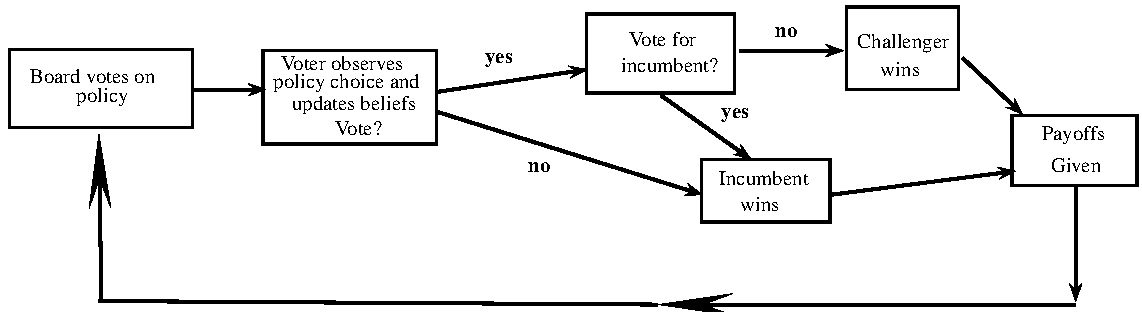
\includegraphics[width=.9\textwidth]{img/wumodel}
\end{figure}
\end{center}

\subsubsection{Policymaking}
The policymaking and political activities of boards remain largely unexplored areas as well. Policy preferences and political goals at other levels of government--such as preferences for state and federal government activity--by school boards have received some attention \citep{RefWorks:258}, but from snapshot studies it can only be concluded that boards have mixed feelings about the role of federal, state, and municipal policymakers in schools \citep{RefWorks:262}. \citet{RefWorks:318} indicates that such variation is expected, and not of tremendous interest, but instead it is the conditions under which the feelings of local policymakers toward state and federal policy changes that is of interest--as such change provides policy opportunities. It is known that boards respond differentially to policy making at the state \citep{RefWorks:187} and federal \citep{RefWorks:236} levels. Unfortunately, no hypotheses about the preferences of boards over state and federal policies have been tested in these studies because the policies tested were broad reform packages covering many issues along multiple dimensions in education policy. 


\subsubsection{Interest Groups}
The role of interest groups and elites in school board politics has also only received a cursory look \citep{RefWorks:254}. \citet{RefWorks:217} have done limited work on the role of public interest groups in school board elections demonstrating that teacher unions, parent groups, business interests, religious, racial, and ethnic organizations all influenced school board elections through canvassing, campaign contributions or both. This is purely descriptive work based on self-reports by surveying school board members serving in office. By surveying winners and losers from school board campaigns \citet{RefWorks:218} found significant influence of teacher unions over the outcome of elections \citep[see also:][]{RefWorks:320,RefWorks:207}. Challenger emergence itself has been explored only in a very narrow scope looking at challengers emerging along a single issue dimension--Christian social values--as well as how these challengers are externally supported \citep{RefWorks:240,RefWorks:347}. Unfortunately these conclusions are not generalizable to whether and when other interest groups encourage and support candidates for school board. This lack of scholarship is surprising because \citet{RefWorks:242} found that when school boards in Virginia moved from being appointed to elected local interest groups viewed elected boards as a new window of influence on school decisions \citep[see also][]{RefWorks:315}. 



\subsection{Board and Superintendent Relationships}

It is nearly impossible to talk about the role of school boards in setting school policy without talking about the relationship between the board and the superintendent. A large portion of the school board literature remains focused on the question of the optimal relationship between board members and the district administrator \citep[see][]{RefWorks:233,RefWorks:263,RefWorks:227,RefWorks:251,RefWorks:229,RefWorks:234,RefWorks:257,RefWorks:264,RefWorks:226,RefWorks:316}. Most of these studies have sought to identify the ideal role of school board members as viewed by superintendents as in \citet{RefWorks:229,RefWorks:234}, or the ideal role of a superintendent as viewed by board members as in \citet{RefWorks:227, RefWorks:233}, or the dynamic between administration and the board \citet{RefWorks:251, RefWorks:257}. 

Unfortunately, there is no application of basic theories of the role of an executive to the relationship between boards and superintendents, though \citet{RefWorks:251} classified the relationships between boards, superintendents, and the community for Wisconsin school districts. Despite trust between the superintendent and the board being identified as a critical component of functional local governance \citep[see][]{RefWorks:229,RefWorks:234,RefWorks:227,RefWorks:233}, spatial models have received only a brief mention in reference to the relationship between the board and superintendent. \citet{RefWorks:340} noted that gathering information for policy action is costly to school board members if conducted independently, and thus in most cases on most policy issues, board members are dependent on the superintendent. Such a spatial model could be critical in providing the link from board turnover to superintendent turnover that dissatisfaction theory seems to expect--see the descriptive studies of \citet{RefWorks:311} for an example. Qualitative work in New Jersey has indicated that a breakdown of trust and mismanagement of the budget are key factors in school boards choosing to buy out a superintendent contract--both activities that tie directly to the informational dependency of the board on the superintendent \citep{RefWorks:246}. 

In essence, the literature has not seriously considered whether to view the district administrator as an executive interacting with a legislative body or as a trusted advisor guiding an executive council. Classifications of board and superintendent relationships have tended to focus on style as in \citet{RefWorks:251} and not on the functional relationship as it relates to policy making. A focus on this relationship is critical to understanding the politics of school districts. 



\section{Proposed Study}
As demonstrated above, the existing literature on school boards has been predominantly theoretical, largely descriptive, or based on case studies of particular board policies and behaviors. Of particular interest to political science has been the level of participation and contention in local elections of school boards. However, the primary theories of school board politics—--continuous participation, dissatisfaction, and decision-output theories—--have only been subjected to limited empirical testing. Recent political events in Wisconsin have created a number of opportunities for research into the causal mechanisms behind school board electoral participation and, school board policymaking.

The election of Scott Walker as Governor of Wisconsin in November 2010 brought sweeping and unexpected changes to education policy in the state of Wisconsin. Among the major changes that are relevant for this study:
\vspace{-12pt} %for anything over single space
\begin{enumerate}
\begin{singlespace}
\item Limitations on the collective bargaining rights of public employee unions including teachers' unions. \footnote{ This in the form of the ``budget repair bill'' known formally as \href{http://docs.legis.wisconsin.gov/2011/related/acts/10.pdf}{2011 Wisconsin Act 10} passed on March, 11 2011.} This includes the elimination of bargaining over the gross wage scale and the restriction on any bargaining over compensation to an annual increase no greater than the increase in the Consumer Price Index (CPI).
\item A dramatic reduction in state aid to school districts for general education revenues in the 2011-2013 Biennial Budget known as 2011 Wisconsin Act 32. \footnote{ The cut was the second largest single-year reduction in per pupil spending in 2010-11 across 46 states studied according to \href{http://www.cbpp.org/files/9-1-11sfp.pdf}{a report} from the Center for Budget Policy and Priorities.}
\item Restrictions on district revenue raising including a reduction in the revenue limit per pupil, elimination of certain expenditures from inclusion in the revenue limit, and a reduction in state categorical aid programs by 10\%\footnote{ The Wisconsin Department of Public Instruction has a strong summary of the 2011-13 budget's impact on school finance \href{http://dpi.wi.gov/pb/11-13_budget.html}{available online}.}
\item A reduction in the levy rate for local property taxes in most school districts statewide, a 1\% decrease in the school tax share of property taxes, and a statewide reduction of \$228 million in property tax rates.\footnote{More information available here: http://www.reforms.wi.gov/section.asp?linkid=1779\&locid=185}
\end{singlespace}
\end{enumerate}

\textbf{This has led to:}
\vspace{-12pt}
\begin{enumerate}
\begin{singlespace}
\item Recall elections against six sitting state senators in the summer of 2011.
\item An unprecedented level of public political activity including weeks of protests in February and March 2011 and an eventual successful petition drive to force a recall election in 2012
\item The politicization of the relationship of teachers to management, and of education expenditures and school district budgets
\item Recall elections against state senators, the lieutenant governor, and the governor on June $5^{th}$ of 2012
\end{singlespace}
\end{enumerate}

Figure \ref{wiscotimeline} shows the interaction between regularly scheduled spring elections, special elections, and the major events enumerated above. This timeline shows that the school board elections in both 2011 and 2012 (Spring elections) had the potential to be influenced by the political turmoil at the state level. However, it is clear that the 2012 election has had more policy shock treatment, as the 2011 spring election occurred in the midst of historic protests and before the outcome of the state budget vote was known. Next, more detail will be provided about the expected relationship between these state level political events and local election results. 

\clearpage
\begin{center}
\begin{figure}[h!]
\caption{Wisconsin Politics 2011-2013 Timeline}
\label{wiscotimeline}
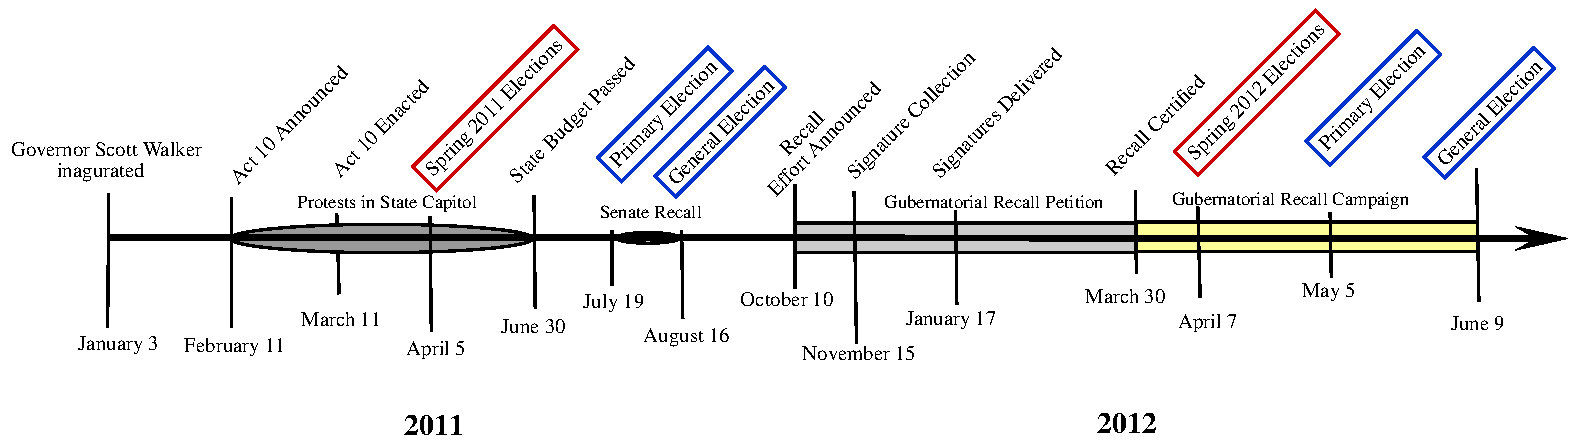
\includegraphics[width=\textwidth,height=1.75in]{img/wiscotimeline}
\end{figure}
\end{center}
\vspace{-48pt}


\subsection{Research Questions and Methodology}
Given the timeline in Figure \ref{wiscotimeline} it is clear that Wisconsin serves as a natural laboratory to explore a few critical questions regarding the relationship between local domain specific elected offices, like school boards, and the state level policies and political climate that they are constrained by and operate within. Specifically, the research questions proposed for this study are:

\vspace{-6mm}
\begin{enumerate}
\begin{singlespace}
\setlength\itemsep{-6pt}
\item How does a state level policy shock affect the level of participation in school board elections both in terms of voter turnout and in terms of challengers to incumbent board members?
\item How does that shock change school board policymaking and what are the predictors of that change in the board?
\item Does sudden partisan polarization of state level politics lead to polarization of school boards along partisan dimensions?
\end{singlespace}
\end{enumerate}
\vspace{-3mm}

While there may be concern that focusing on one state is too constraining to be generalizable or theoretically interesting, the unique leverage directly on the above questions in the Wisconsin case will be demonstrated below. In areas like school board elections where little theory development has occurred, \citet{RefWorks:192} argue that the literature may best be served by the more in-depth and comprehensive study of a smaller system that a single-state study like that proposed here can provide. Furthermore, the foundational study on critical elections was in essence an in-depth case study of electoral behavior in key areas \citep{RefWorks:348}.

Wisconsin provides an excellent laboratory for exploring these three issues because of the high salience of education issues in a newly polarized political climate. The state level policies that have led to these conditions were more or less unanticipated by voters, school boards, teachers' unions, and other strategic actors due to the little attention paid to either the budget allocation for schools or the rollback of public employee bargaining rights in the 2010 gubernatorial campaign in Wisconsin.\footnote{This last point is somewhat disputed by some political observers and Scott Walker himself, but the consensus has been that this was not the case according to the \href{http://www.politifact.com/wisconsin/statements/2011/feb/22/scott-walker/wisconsin-gov-scott-walker-says-he-campaigned-his-/}{Milwaukee Journal Sentinel}.} Additionally, the reforms enacted by Governor Walker give school boards unprecedented new freedom to radically rethink district policy, organization, and employee compensation--thus removing a substantial constraint on the potential policy preferences of school boards. This provides an opportunity for both a rigorous test of hypotheses about influence of state politics on local elections due to the exogenous nature of the policy shock, and an opportunity to explore the shift in interest group power as school boards were given unprecedented freedom in drafting employee contracts. 

Figure \ref{model} provides an overview of how these questions might fit together. In the pre-election period school boards make policies, interest groups organize, and voters form strong preferences about their approval of the Governor's education reforms.\footnote{Strong here denotes only that the preferences are strong relative to voter preferences for school board candidates--a fairly weak assumption.} In this period we expect board policy to be influenced by their perceptions of the strength of interest groups, district consensus supporting the Governor's reforms, and overall support for the Governor. Local level policy concerns much as in \citet{RefWorks:243}, in turn, then influence both emergence of challengers and voter participation. Thus, the board makes policy like how to allocate limited resources--as a response to the budget cuts almost all districts received, how to compensate employees, and whether or not to extend teacher union contracts all in anticipation of their view of voter and interest group strength and support for those policies. As in \citet{RefWorks:243} when boards choose correctly and align policy with community preferences, then few challengers should emerge, turnout should be low, and the board will remain intact. However, if boards either misjudge the preferences of voters in their policies, or if voters are sharply divided, then the number of challengers should increase, and boards should experience turnover. The result of board turnover is superintendent turnover and potentially student achievement, both of which creates a feedback loop shaping future education policy and pre-election activity \citep[see][]{RefWorks:345,RefWorks:297,RefWorks:271,RefWorks:311}.

\begin{center}
\begin{figure}[h!]
\caption{A Theoretical Model of School Board Policy Shock}
\label{model}
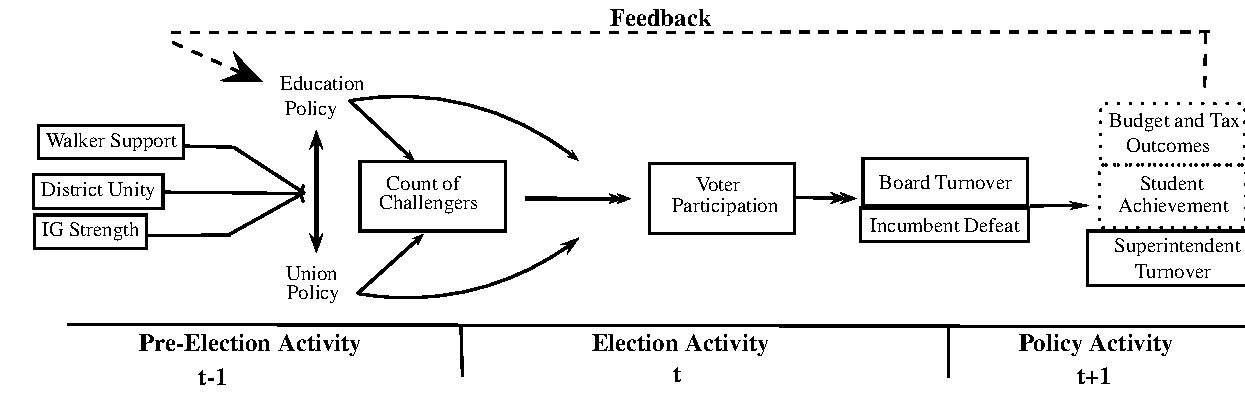
\includegraphics[width=.9\textwidth]{img/theory}
\end{figure}
\end{center}
\vspace{-48pt}

In the models that follow the results of the 2011 Gubernatorial Recall Election are used in one of two ways. First, the results are used to show community unity around the Governor's education policies. The larger the vote share either for or against the Governor (i.e. the further away from 50\% the Governor's vote share is), the more community consensus around these education policies is believed to exist--either in support or opposition. Second, the results are used to show overall community support for the Governor's education policies in lieu of the ability to poll community members in every school district. The larger the vote share for the Governor, the more it is assumed that voters support the Governor's policies, and the more likely it is that a plurality of voters in the Spring Election also support the Governor's policies. Thus, the close timing of the recall election to the spring elections allows one to safely assume that the recall election results serve as an instrument for voter support for or against the Governor's policies in the spring election as well. It is this unique leverage on the preferences of voters that all of the following models take advantage of to show how voter preferences shape features of the spring elections. 

\subsection{Candidate and Voter Participation}
Did Governor Walker's polarizing and dramatic policy changes lead to increased participation by candidates and voters in spring elections? Leveraging this deeply partisan exogenous shock to education policy in the state, it is possible to evaluate if spillover from such events leads to increased activity in elections held at a different level of government. Wisconsin school board members are elected in spring elections which have no candidates for a partisan statewide office--though county level offices are present as are non-partisan offices like State Supreme Court and Superintendent of Public Schools. For both candidate and voter participation I will use data on turnout and election returns from several prior elections to estimate the long term trend in participation in terms of voter turnout and the number of candidates, especially challengers to incumbents, and then use a regression model to estimate the impact of policy in 2011 on both. 

\subsubsection{Candidate Participation}
\label{sec:ce}
Running for school board, while typically not financially burdensome, is burdensome in terms of time and energy \citep{RefWorks:336}. Additionally, school board service often requires long hours, is predominantly unpaid or nominally paid, and requires giving up many weeknights for public meetings \citep{RefWorks:333}. Moreover, despite a few high profile exceptions, the school board has not been found to be a stepping stone office for career politicians \citep{RefWorks:333}. Yet, candidates emerge. \citet{RefWorks:336}'s application of public choice theory to school board members implies that more challengers should emerge when deep policy divisions exist within a community over issues that matter to the public. 

The environment in Wisconsin is ripe for just such a test, because some communities are unified on one side or the other of Governor Walker's reforms, while other communities remain deeply divided. In districts that are unified fewer challengers should emerge for school board, and in divided communities, more school board seats are expected to be contested. Using election returns for school board elections in school districts across the state it is possible to evaluate the long-term trends in contested school board seats and compare that to the elections in the Spring of 2012. Additional followup with individual school districts could check for the prevalence of politically motivated retirements where incumbents stand down rather than engage in a costly election against a strong incumbent--an issue identified previously in the literature as confounding \citep{RefWorks:311}. 

Combining this information with returns from the late spring recall election of the Governor--certain to be a statewide referendum on the Governor's education policies--it is possible using data from all 424 school districts in the state to directly to test whether divided communities see greater participation by challenger candidates than unified communities. This would represent the first comprehensive test of the public choice theory of school board elections and represent the first test of Dissatisfaction Theory across an entire state using actual election results instead of self-reports of school board members and superintendents \citep{RefWorks:243,RefWorks:297}. The empirical model of candidate emergence (CE) would look something like: \\

$(1)  \hspace{2 in}  CE_{t} = \alpha + \beta X_{t-1} + \gamma Z_{t} + \epsilon $ \\

Where $CE_{t}$ represents a measure of the number of candidates greater than one per seat, $\alpha$ is an intercept, $X_{t-1}$ is a vector of lagged covariates such as prior levels of contestation and district size, and $Z_{t}$ is the absolute value of the deviation from 50\% of the vote share for the Governor in a recall election aggregated to the school district from ward level returns.\footnote{Depending on the data and the prevalence of incumbent retirements candidate emergence may need to be measured a number of additional ways. \citet{RefWorks:337} discuss a number of possibilities for turnover that could be adapted to candidate emergence including: Seats available divided by incumbents + challengers minus retired candidates; seats available divided by all candidates; or seats available divided by challengers.} Thus, when $Z_{t} = 0$ the community is completely divided on the Governor. When $Z_{t}=.5$ the community is either united for or against the Governor. Thus, all things equal, we would expect $\gamma$ to have a negative value--as $Z_{t}$ increases, the number of challengers, $Y_{t}$ should decrease because the community is fairly homogeneous and the school board should reflect existing preferences for or against the Governor's reforms. 

\subsubsection{Voter Participation}
\label{sec:vp}
Political science has long noted that turnout increases in elections with an ``up-ticket'' candidate, most notably a president. However, in the 2011 and 2012 spring elections in Wisconsin it is not an up-ticket candidate, instead there is a deep shift in the political climate of the state. Do school board elections exhibit increased turnout in response to policy shocks from the state level and/or increased polarization? All the major theories predict that voter participation should increase in Wisconsin, but by working with additional data, it becomes possible to gain insight into what is driving those changes by taking advantage of the natural variation in conditions across the entire state. Dissatisfaction Theory predicts that voter turnout increases when the school board's policy decisions are out of line with the preferences of the community to a substantial degree \citep{RefWorks:297}. Continuous Participation Theory predicts that participation in school board elections is an elite-driven affair and that participation increases when the minority that continuously participates in elections seeks support from the electorate \citep{RefWorks:283}. Finally, Public Choice Theory suggests that voters only participate when the perceived benefit from a candidate's policy positions exceeds the cost of voting \citep{RefWorks:336,RefWorks:243}. 

To disentangle these predictions it is necessary to understand board responses to Governor Walker's policies, interest group preferences for board members, and public preferences for Governor Walker's reforms in school districts. Contrasting the predictive power of each of these variables in relation to the change in turnout in the spring elections of 2011 and 2012 compared to prior years will help better understand which of the theories are appropriate and when. This empirical model for voter participation would look something like: \\


$(2) \hspace{0.8 in} VP_{t} = \alpha + \beta X_{lag} + \gamma W_{t} + \lambda P_{lag} + \tau 1- |W_{t} * P_{lag}| + \theta I_{lag} + \psi Ce_{t}+\epsilon$\\

Here $VP_{t}$ is voter turnout in either the 2011 or 2012 Spring Elections by school district in Wisconsin. $\alpha$, $X_{lag}$ remain the same as above though now including some measure of prior turnout in the district such as turnout in the Gubernatorial election in 2010. $P_{lag}$ represents the direction of policy changes, if any, taken by the board in relation to the Governor's reforms--where 1 is an elimination of employee contracts and -1 is resistance to the Governor's reforms in the form of extending union contracts.\footnote{This measure will only be available for a subsample of districts due to the fact that some districts were unable to choose to end their contracts due to remaining years of obligation.} $I_{lag}$ representing an indicator of the strength of teachers' unions in the district--likely the most salient and relevant interest group in the spring elections \citep{RefWorks:320, RefWorks:207, RefWorks:218}.\footnote{This may prove unobservable, buta numer of potential variables exist: for example, the number of grievances filed per member on behalf of the local union over the last several years using the grievance database available from the Wisconsin Employment Relations Commission (WERC), votes for union recertification in a subsample of districts, campaign contributions by teachers by school district, though each of these measures carry other meaning as well}. Voters are unlikely to participate if presented with no choice, so $Ce_{t}$ represents a measure of the number of candidates per seat. $W_{t}$ represents the vote share for Governor Walker in the recall election--a measure of community support or opposition to the Governor's education policy. Thus it would be expected that $\theta$ should be positive--strong interest groups should drive political activity. The inclusion of partisanship predictors of voter turnout could also be explored here. The effects of $\gamma$  and $\lambda$ alone are uninteresting, but the interaction of $W_{t} * P_{lag}$ is of great interest. This essentially represents a measure of board policy alignment with voter preferences--taking the absolute value simplifies interpretation. As such, it should be expected that for large values of $W_{t} * P_{lag}$, voter participation would be small as the board policy and the community preferences would be aligned. As $W_{t} * P_{lag}$ approaches zero, voter participation will increase as predicted by \citep{RefWorks:243}--voters seeing dissonance between their preferences and board policy are more likely to vote. Thus $\tau$ should be negative.  %Add detail here

Unlike with candidate participation, the voter participation analysis does have a potentially serious confounding factor. In 2012 there is a Presidential Preference Primary which, due to the competitive Republican presidential primary in 2012, is a competitive election relevant to the Spring electorate. Thus, this analysis will be unable to disentangle increased voter turnout for school board elections in the Spring of 2012 due to Governor Walker's policies from voters' desire to pick the Republican candidate for President. There are some strategies to mitigate this problem; including comparing the analysis to 2008 voter turnout when an unusually long Democratic primary made the presidential primary relevant as well, controlling for unity among the presidential candidates on the ticket, or controlling for a rolling average of voter turnout across several election types to capture a district's propensity to participate across different electoral conditions. 

\subsection{Board Policy Responses}
\label{sec:bp}
In the wake of Governor Walker's reforms school boards were faced with two immediate policy concerns. First, many boards had the choice to extend employee contracts to preserve existing collective bargaining agreements or to dissolve those agreements and develop a new employee compensation scheme under the new rules established in state law. Second, boards had to decide how to balance their budgets and raise revenue under the new conditions established by the Governor's state budget.\footnote{Note that almost all districts saw a steep reduction in their funding from 2010 to 2011 as a result of Governor Walker's budget.} Both policies were extremely high profile for school boards often garnering attention in local newspapers. 

Board responsiveness has previously only been studied in case studies looking at individual school districts or a small sub-sample of school districts in a state \citep{RefWorks:253,RefWorks:236}. Such attempts were plagued by an inability to identify common policy issues to evaluate movement along, or an obvious ideological divide to compare board members and boards. Wisconsin presents an opportunity to study board choices on policy in response to highly salient state reforms systematically--a rare opportunity as most state level policy that boards must consider is of low salience to voters and often of a technical nature, like the adoption of state or national curriculum standards.As a result of state policy in 2011 boards have already begun revisiting their employee compensation plans. Some boards have chosen to extend existing employee contracts and employee handbooks as far into the future as possible to preserve previously bargained agreements between employees and the districts, while other districts have scrapped their prior collective bargaining agreement and renegotiated compensation with employees under the new rules established by the state. A final set of districts had existing contracts that extended into 2013 and could not extend them further. 

To analyze the responsiveness of boards to policy preferences of their constituents it is necessary to evaluate the policies systematically. Data on boards scrapping, keeping, and locked into their employee compensation agreements have already been collected. Then, once a theoretical expectation about why boards would make a particular choice is developed the predictive power of that theory can be tested. From informal conversations with members of the Wisconsin Association of School Boards (WASB) and Wisconsin Association of School District Administrators (WASDA) it seems clear that boards extended contracts in places where they felt political support was high for teachers' unions and scrapped contracts where they felt public support favored lower taxes. Thus, the analytical model for union policy might look something like:\\

$(3) \hspace{2 in} UP_{i} = \alpha + \beta X_{lag} + \gamma Z_{t} + \theta I_{t} + \epsilon$ \\

Where $UP_{i}$ is an indicator -1 for scrapping the contract, 0 for being locked in (or dropped from the sample), and 1 is extending the contract. $\alpha$, $X_{lag}$ remain the same as above. $Z_{t}$ is now the vote share of Governor Walker in the recall election, a measure of community support for his policies, while $I_{t}$ is a measure of union strength using data obtained from the Wisconsin Employee Relations Council (WERC) on employee votes for and against union re-certification--a clear signal to the school board of union strength. Note that this model is anticipatory--did boards correctly respond to the community's preferences which were revealed by $Z_{t}$ and  $I_{t}$ a few months later? The expectation is that $\theta$ should be positive--as union strength increases so does the likelihood the board extends collective bargaining agreements. Logically, $\gamma$, the coefficient on Governor Walker's vote share should be negative, the more support for the Governor in a district, the more likely an anticipatory school board would be to eliminate the union contract. The expected interaction between $\gamma$ and $\theta$ will have to be explored in more detail before any definite hypotheses about this relationship can be made. The staggered nature of school districts' existing contracts means only a subsample had the option of extending or not extending their contract and resisting Act 10. Thus this analysis will not include the full sample of school districts.\footnote{A further complication is that school districts making this decision faced a tension between needing to decide budget decisions for the next school year, but being unsure due to the political turmoil in the state about the permanency of their ability to set employee compensation policy outside of a union contract.}

While the collective bargaining issue is staggered with the length of existing employee contracts, districts faced the change in their fiscal situation at the same time. DPI and the Wisconsin Association of School District Administrators have collected detailed information on the responses of nearly every district in the state to such fiscal tightening in 2011 and plans to gather such information again in 2012.\footnote{The original survey form for 2011 and for 2012 can be found online: http://dpi.wi.gov/eis/pdf/wasdasurvey.pdf} These data provide a snapshot of the policy decisions made by school boards including tough decisions about what subjects and programs to cutback or eliminate. This empirical model for evaluating budget policy decisions might look something like: \\


$(4) \hspace{2 in} B_{i} = \alpha + \beta X_{lag} + \gamma Z_{t} + \theta P_{lag} + \epsilon$\\

$\alpha$, $X_{lag}$, and $Z_{t}$ remain the same as above. $B_{i}$ is an indicator of the depth or the breadth of budget cuts in a district relative to its size and $P_{lag}$ is a set of budget cut specific control variables such as the district having a budget referenda or other factors mitigating the depth of budget cuts like federal stimulus aid or unused revenue limit authority. 

Data on school district budgets is fairly comprehensive and can be acquired from a number of sources. This data includes specific details about the types of positions, types of programs, and types of revenue decisions school districts made in response to the sharp decrease in state aid and revenue limit authority available to support school district operations. It also includes information about the maximum tax base available to the district, and the maximum levy available to assess for funding school operations. 

\subsection{Partisanship in Board Elections}
\label{sec:pid}

\textbf{Note: This part of the project will not be part of the dissertation, but is a very likely additional paper/extension of the project later.}

Wisconsin school boards are non-partisan offices. Previous research has shown that board members are typically a moderate bunch when asked to self-identify their political ideology \citep{RefWorks:321,RefWorks:333}. However, relying on self-assessments of officials holding a non-partisan office is not a reliable measure of the political leanings of board members. Unfortunately, finding a valid external measure of board member ideology or partisanship has been previously impossible in non-partisan board elections--making member self-reports the only available data. 

Again, the situation in Wisconsin provides unique leverage on this question. Of school boards with the option to extend contracts to teachers' unions, all school board members had to publicly vote in support of or against the extension of the contract on the record at a public board meeting. These votes, like all official board votes, are recorded in the minutes of the board meeting and available for the public to review. Board members were under no illusion that this vote was anything other than a statement of public support or opposition for Governor Walker, a Republican. While this measure is not necessarily indicative of a board member's political leanings on other issues, it is a public signal of partisanship to the electorate. The ability even to simply describe the partisan makeup of the majority of school districts for a single year is of great interest to compare to findings from national surveys and surveys in other states.

However, the study can go a step further with some basic assumptions. To understand the partisan makeup of Wisconsin school districts before and after the Spring elections, the votes of all board members for and against extension of employee union contracts will be collected and then for those facing re-election the outcome of their Spring 2012 election will be coded.\footnote{Or a sample will be drawn depending on the difficulty of collecting the data and the number of board members in the population of interest.} Then an empirical model of partisanship looks something like this:\\

$(5) \hspace{2 in} PID_{i} = \alpha + \beta X_{lag} + \gamma Z_{t} + \epsilon$ \\

$\alpha$, $X_{lag}$ remain the same as above. $Z_{t}$ is again the vote share for Governor Walker. Here $PID_{i}$ represents the change in partisanship of the board from before and after the Spring 2012 election in terms of direction and magnitude of seat swings on the board. For example, if the board had five members, two supportive of the Governor's policies and three in opposition, the board would be -1 in terms of the strength of support for the Governor. Thus, $\gamma$ is expected to be positive, with more community support for Governor Walker translating into an increase in the number of seats filled by board members also supportive of the Governor's policies.  

This analysis will rely on the assumption that a board member who is defeated is defeated by a candidate with an opposite position on extending union contracts. If this assumption appears too dubious the sample could be reduced to a size where the position of both candidates could be verified in all elections by reviewing local newspaper coverage of the elections. And, it should be noted, this analysis will only be possible if two conditions are met: that the results of these votes can be reliably located and that boards exhibited significant enough public contestation over such votes--neither of which are known at this time.

\subsection{Summary of Questions, Hypotheses, and Models}

Table \ref{hypotab} summarizes the variables of interest and their expected influence on the dependent variable from the models above in sections \nameref{sec:ce}, \nameref{sec:vp}, \nameref{sec:bp},and \nameref{sec:pid}. 

\begin{table}[h!]
\begin{center}
\begin{small}
\caption{Summarizing Hypotheses}
\label{hypotab}
\begin{tabular}{| p{.25\textwidth} | p{.4\textwidth} | p{.25\textwidth} |}
\hline
\textbf{Dependent Variable}  & \textbf{Independent Variable} & \textbf{Expectation} \\ \hline
\multirow{2}{*}{Candidate Participation} & Unity on State Policy ($\uparrow$) & Negative \\ & Previous Challenger Emergence $(\uparrow)$ & Null \\ \hline
\multirow{4}{*}{Voter Participation} & Prior Turnout $(\uparrow)$ & Positive \\ & Number of Challengers $(\uparrow)$ & Positive \\ & Interest Group Strength $(\uparrow)$ & Positive \\
                & Policy Divergence $(\uparrow)$ & Positive \\ \hline
\multirow{2}{*}{Union Policy} & Union Strength $(\uparrow)$ & Policy Resistance \\ & Governor Walker Support $(\uparrow)$ & Policy Support \\ \hline
\multirow{2}{*}{Budget Policy} & Budgetary Health $(\uparrow)$ & Fewer Cuts \\ & Governor Walker Support $(\uparrow)$ & Greater Cuts \\ \hline
\end{tabular}
\end{small}
\end{center}
\end{table}

The specific statistical method to produce estimates for each of these models will depend on the quality and breadth of data made available as well as the final transformations applied to dependent variables. As is detailed below, it is not yet known what the extent of reliable historical election records is statewide in Wisconsin for spring election results. All results for local offices are the responsibility of county election clerks in Wisconsin for each of the 72 counties. Fortunately, there exist a number of county election clerks who are also school board members, and in my talks with the Wisconsin Association of School Boards they have indicated that these members are willing to help me in navigating access and requests to each of the 72 counties. Still, there is no clear state records retention policy for each county, so at this time I am unable to know the historical extent of variables for electoral participation by school district. It may be the case that comparisons can only be made in recent years by using previous Gubernatorial election results and the corresponding spring election years such as the 2010 election of Scott Walker or the 2006 re-election of Democratic governor Jim Doyle. 

\subsection{Data and Design}

I plan on collecting in depth data on school board elections in the state of Wisconsin. Combining these data with longitudinal data on student achievement, district financial outcomes, superintendent tenure, and policy changes within districts will create a more comprehensive picture of the nature of school board elections and decisions than has been done previously. A cursory review of the data elements required to be collected and where they can be found is given below:
\begin{enumerate}
  \item \textbf{Longitudinal student achievement data.} This data is available from the Wisconsin Department of Public Instruction for all students in the state from 2005-2006 to present. This data is readily obtained for all students tested by state achievement tests in grades 3-8 and 10. It also includes basic demographic characteristics of public school students and additional information on attendance and disciplinary incidents. This data is readily obtained through the DPI's research request process.
  \item \textbf{School board and superintendent turnover.} The Wisconsin DPI has collected information on names of the school board members, school board president, and school district superintendent is each school year since 2002-2003. 
  \item \textbf {Election results for school board members.} This data is collected by the clerk for each school board and then reported to each of Wisconsin's 72 counties. These data are not available in a digital format online for all districts or for all time periods. Acquiring this data will take a significant amount of time and will involve contacting each county election clerk directly, possibly paying for copies of election returns, and entering election returns into a database. Ideally election results would include vote share for each candidate for each school board seat, as well as overall voter turnout in the election. I will request results from 1994 to present. %citation
  \item \textbf{Gubernatorial Election Returns.} Ward-level election returns in the recall election of Governor Walker can serve as a statewide opinion poll on the policy shock of interest. Using this data as an indicator of the level of support in a community for the state level policy shocks is vital in evaluating the ideological position of school boards in contrast to their communities. This data will be made available after the election by the Government Accountability Board.\footnote{A possible complication is the legal wrangling over when new electoral districts are drawn which changes only how the data is referenced for a statewide election--using 2000 data and wards or 2010 data and wards.} For comparison, returns from the 2010 and 2006 Gubernatorial elections as well as the 2008 presidential election will be collected as well.
  \item \textbf{District Budgetary Data.} There are two major sources of budget data about school districts. The first is the 2011 Budget Cut Survey conducted by the Wisconsin Association of School District Administrators (WASDA) and analyzed by the Wisconsin DPI.\footnote{http://dpi.wi.gov/eis/pdf/wasdasurveyresults.pdf}. This survey includes detailed questions about what types of positions districts cut and in which areas of operations, as well as class size increases and their outlook for fiscal health in the future. This survey will be reissued in the fall of 2012 as well. 88\% of districts responded and a similar response rate is expected next year. The second major source of data is the DPI school financial database, which is used to calculate state aid allocations to school districts and to monitor school district finances. This includes a wide arrange of information from 1995 to present on school district revenue sources, expenditures, and tax rates. It also includes the results of all school budget referenda including the votes for and against and the size of the levy being voted on.
  \item \textbf{Board policy decisions.} General data about collective bargaining contract negotiations will be obtained by working with the Wisconsin School Board Association and the Wisconsin Association of School District Administrators; I have strong relationships with both organizations. This data will include the length of the contract, whether the board extended the contract in response to state-level reforms, and the number of times contract negotiations have gone to arbitration in the previous decade. More detailed data such as board meeting minutes and records of board member votes to extend contracts would be restricted to a small sample of districts, perhaps 10\% of districts in the state, and only in years in which student data is available--because historical records may not be available.
\end{enumerate}


